\newcommand{\numTD}{TD3}
\newcommand{\themeTD}{Clustering avec un algorithme d'affinité de propagation}
\newcommand{\file}{toto.tex}

\begin{center}
\begin{tabular}{|p{2cm}p{14cm}|}
\hline
{
\includegraphics[width=1.8cm,viewport=0 0 337 248]{../CM/images/sorbonne.png}} & \raisebox{2ex}{\begin{Large}\textbf{Programmation de Modèles Linguistiques (I)}\end{Large}}\\

%2019-2020& \raisebox{2ex}{\begin{large}\textbf{L5SOPROG L3 Sciences du Langage}\end{large}}\\
2023-2024& \raisebox{2ex}{(L5SOPROG L3 Sciences du Langage)}\\
   & \begin{large}\textbf{\numTD}\end{large} \begin{large} \textbf{\themeTD}\end{large} \\
&\\
& Caroline Koudoro-Parfait, Sorbonne Université \\
\hline
\end{tabular}
\end{center}


\hrule
%%%%%%%%%%%%%%%%%%%%%%%%%EN-TETE%%%%%%%%%%%%%%%%%%%%%%%%%%%%%
%\renewcommand{\contentsname}{Sommaire du TD}
%\tableofcontents
%\newpage

\noindent\fcolorbox{lightgray}{lightgray}{

\begin{minipage}{12cm}
\section*{Objectifs}
\begin{itemize}
 \item Créer un compte Github
 \item Utiliser Github desktop
 \item récupérer en local un dépôt existant sur le serveur
 \item faire des modifications dans le dépôt en local
 \item partager les modifications sur le serveur 
\end{itemize}
\end{minipage}
}
\newline
\section{Avant de commencer}

\begin{enumerate}
\item Le TD se fait en binôme
\item Le binôme définit quel compte servira à créer le dépôt distant contenant le script et quel compte clonera le dépôt distant en local
\item Le binôme récupère le script sur Moodle
\end{enumerate}

\noindent\fcolorbox{red}{lightgray}{IL faut suivre les indications pas à pas car chaque participant du binôme utilise la même branche.}

\section{Créer un compte Github}



\begin{figure}[H]
\caption{\url{https://github.com/.}}
  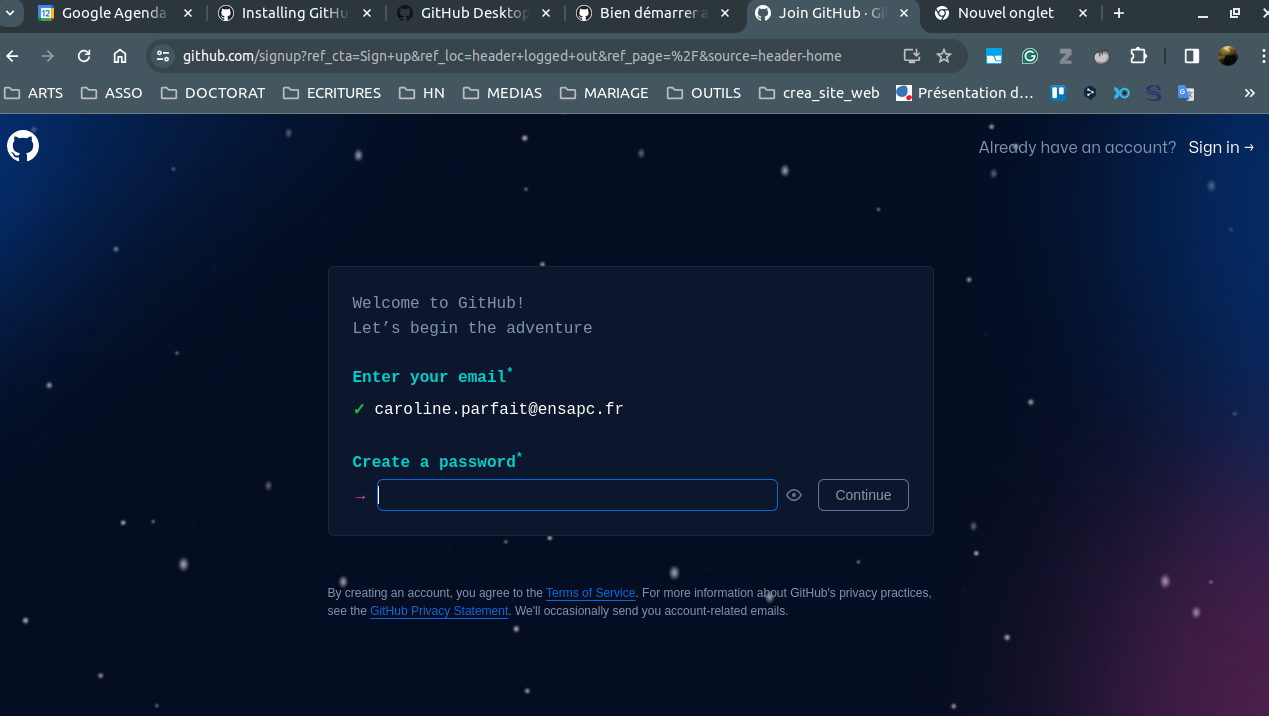
\includegraphics[width=6cm]{images/github_inscription.png}
  
  \end{figure}

\ding{220} Suivre les indications du site web


\vspace{0.5cm}
\section{Télécharger et démarrer avec Github desktop}
\vspace{0.5cm}

\begin{figure}[H]
\caption{\url{https://desktop.github.com/?ref_cta=download+desktop&ref_loc=installing+github+desktop&ref_page=docs}}
  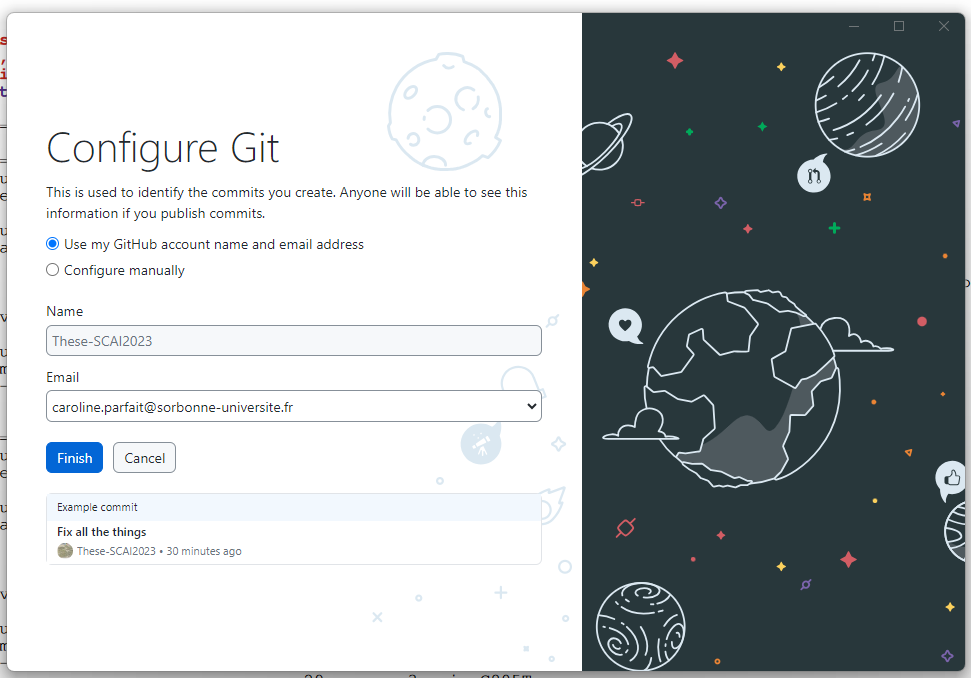
\includegraphics[width=6cm]{images/github_desktop_connect.png}
  
  \end{figure}

\ding{220} Suivre les indications du site web



\section{Créer un dépôt distant sur le serveur}
%\vspace{0.5cm}
La personne du binôme qui doit créer le dépôt distant fait les actions suivantes :

\begin{enumerate}
\item Sur la page "repositories" de votre compte cliquer sur le bouton vert "New"
\item compléter la page en donnant un nom à votre dépôt
\item Laisser le dépôt en "Public"
\item ajouter un README qui sert à la description du programme/la documentation.
\end{enumerate}
  

\begin{figure}[H]

  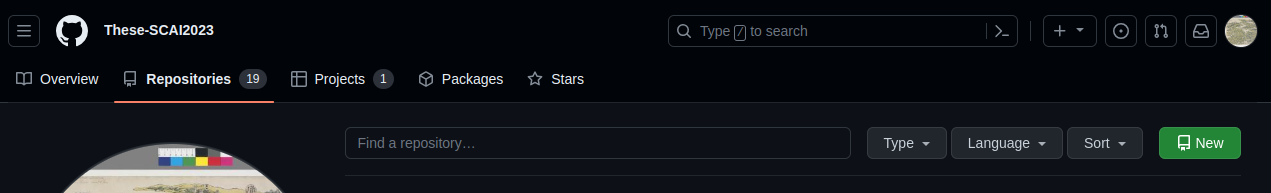
\includegraphics[width=10cm]{images/depot_distant_crea.png}
    \end{figure}

\begin{figure}[H]

  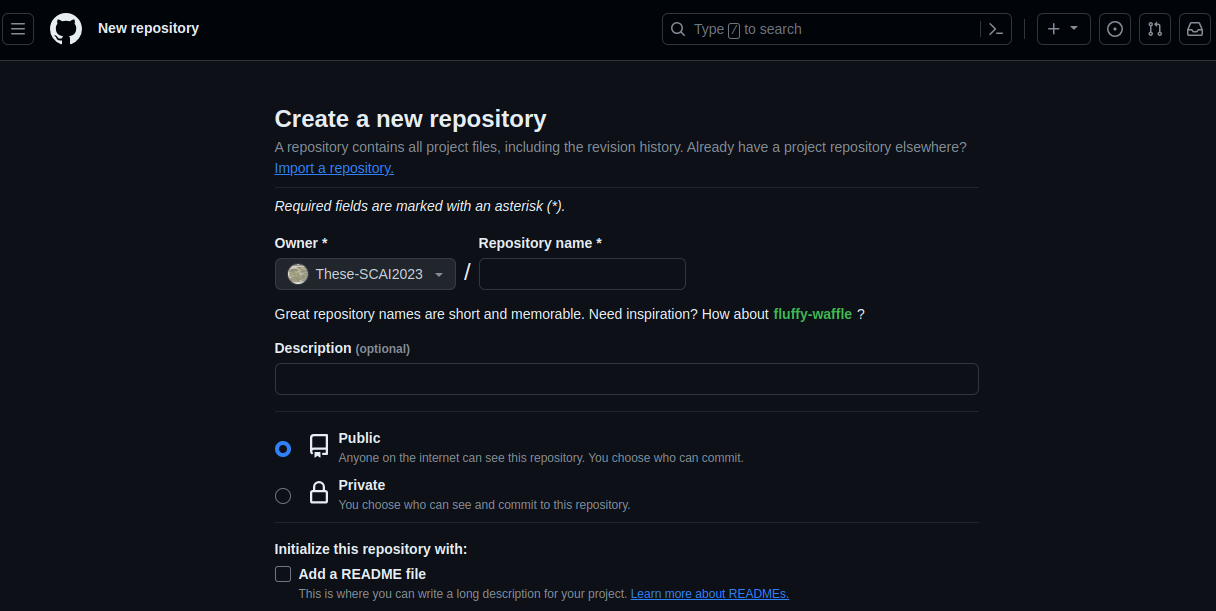
\includegraphics[width=10cm]{images/depot_distant_crea2.png}
    \end{figure}

\section{récupérer en local un dépôt existant sur le serveur}
%\vspace{0.5cm}
La personne du binôme qui doit cloner le dépôt distant fait les actions suivantes :


Pour cloner le dépôt vous pouvez SOIT :
\begin{itemize}
\item  vous rendre sur la page du dépôt
\begin{itemize}
\item cliquez sur le bouton vert "code" 
\item cliquez "ouvrir avec Github Desktop"
\end{itemize}

\item SOIT via l'interface  Github Desktop "clone a repository from the internet"
\end{itemize}


\section{faire des modifications dans le dépôt en local}

Le binôme désigne en amont de toutes actions,
\begin{itemize}
\item L'une des personnes du binôme copie-colle le texte suivant dans le README.md
\item La seconde personne fait une modification dans le script.py
\end{itemize}


\section{partager les modifications sur le serveur}

Suivre pas à pas :

\subsection{Modifier le README}

La personnes désignée par le binôme copie-colle le texte suivant dans le README.md : 


\textit{"Ce programme sert à compter le nombre de tokens appartenant à des entités nommées (EN) dans un fichier CSV. Les EN sont annotées au format IOB2" }

\subsubsection{Commit et Push du README}
Via Github desktop, celui qui a modifié le README.md doit désormais 
\begin{enumerate}
\item "commit", donner une indication pour le commit du type "maj README"
\item push ses modifications
\end{enumerate}

\subsubsection{Pull request}
Le second récupère les modifications en cliquant sur "pull request"

\subsection{Modifier le script}

La personnes désignée par le binôme modifie le script en ajoutant la ligne suivante 

\begin{python}
 print("Il y a",len(liste_EN),"d'entités nommées pour le texte",chemin)
\end{python}
\subsubsection{Commit et Push du README}
Via Github desktop, celui qui a modifié le script doit désormais 
\begin{enumerate}
\item "commit", donner une indication pour le commit du type "maj README"
\item push ses modifications
\end{enumerate}

\subsubsection{Pull request}
Le second récupère les modifications en cliquant sur "pull request"


\begin{center}

\noindent\fcolorbox{blue}{lightgray}{
	\begin{minipage}{15cm}
\section*{Devoir}

\begin{itemize}
 \item 1 script(s) python .py modifié
 \item 1 README.md modifié

\end{itemize}

 
 Envoie par mail du lien vers le Dépôt sur Github : caroline.parfait@sorbonne-universite.fr
 Date limite : 15 mars 2024, 17h.

\end{minipage}
}
	\end{center}
